% Options for packages loaded elsewhere
\PassOptionsToPackage{unicode}{hyperref}
\PassOptionsToPackage{hyphens}{url}
\PassOptionsToPackage{dvipsnames,svgnames,x11names}{xcolor}
%
\documentclass[
  letterpaper,
  DIV=11,
  numbers=noendperiod]{scrartcl}

\usepackage{amsmath,amssymb}
\usepackage{iftex}
\ifPDFTeX
  \usepackage[T1]{fontenc}
  \usepackage[utf8]{inputenc}
  \usepackage{textcomp} % provide euro and other symbols
\else % if luatex or xetex
  \usepackage{unicode-math}
  \defaultfontfeatures{Scale=MatchLowercase}
  \defaultfontfeatures[\rmfamily]{Ligatures=TeX,Scale=1}
\fi
\usepackage{lmodern}
\ifPDFTeX\else  
    % xetex/luatex font selection
\fi
% Use upquote if available, for straight quotes in verbatim environments
\IfFileExists{upquote.sty}{\usepackage{upquote}}{}
\IfFileExists{microtype.sty}{% use microtype if available
  \usepackage[]{microtype}
  \UseMicrotypeSet[protrusion]{basicmath} % disable protrusion for tt fonts
}{}
\makeatletter
\@ifundefined{KOMAClassName}{% if non-KOMA class
  \IfFileExists{parskip.sty}{%
    \usepackage{parskip}
  }{% else
    \setlength{\parindent}{0pt}
    \setlength{\parskip}{6pt plus 2pt minus 1pt}}
}{% if KOMA class
  \KOMAoptions{parskip=half}}
\makeatother
\usepackage{xcolor}
\setlength{\emergencystretch}{3em} % prevent overfull lines
\setcounter{secnumdepth}{-\maxdimen} % remove section numbering
% Make \paragraph and \subparagraph free-standing
\makeatletter
\ifx\paragraph\undefined\else
  \let\oldparagraph\paragraph
  \renewcommand{\paragraph}{
    \@ifstar
      \xxxParagraphStar
      \xxxParagraphNoStar
  }
  \newcommand{\xxxParagraphStar}[1]{\oldparagraph*{#1}\mbox{}}
  \newcommand{\xxxParagraphNoStar}[1]{\oldparagraph{#1}\mbox{}}
\fi
\ifx\subparagraph\undefined\else
  \let\oldsubparagraph\subparagraph
  \renewcommand{\subparagraph}{
    \@ifstar
      \xxxSubParagraphStar
      \xxxSubParagraphNoStar
  }
  \newcommand{\xxxSubParagraphStar}[1]{\oldsubparagraph*{#1}\mbox{}}
  \newcommand{\xxxSubParagraphNoStar}[1]{\oldsubparagraph{#1}\mbox{}}
\fi
\makeatother

\usepackage{color}
\usepackage{fancyvrb}
\newcommand{\VerbBar}{|}
\newcommand{\VERB}{\Verb[commandchars=\\\{\}]}
\DefineVerbatimEnvironment{Highlighting}{Verbatim}{commandchars=\\\{\}}
% Add ',fontsize=\small' for more characters per line
\usepackage{framed}
\definecolor{shadecolor}{RGB}{241,243,245}
\newenvironment{Shaded}{\begin{snugshade}}{\end{snugshade}}
\newcommand{\AlertTok}[1]{\textcolor[rgb]{0.68,0.00,0.00}{#1}}
\newcommand{\AnnotationTok}[1]{\textcolor[rgb]{0.37,0.37,0.37}{#1}}
\newcommand{\AttributeTok}[1]{\textcolor[rgb]{0.40,0.45,0.13}{#1}}
\newcommand{\BaseNTok}[1]{\textcolor[rgb]{0.68,0.00,0.00}{#1}}
\newcommand{\BuiltInTok}[1]{\textcolor[rgb]{0.00,0.23,0.31}{#1}}
\newcommand{\CharTok}[1]{\textcolor[rgb]{0.13,0.47,0.30}{#1}}
\newcommand{\CommentTok}[1]{\textcolor[rgb]{0.37,0.37,0.37}{#1}}
\newcommand{\CommentVarTok}[1]{\textcolor[rgb]{0.37,0.37,0.37}{\textit{#1}}}
\newcommand{\ConstantTok}[1]{\textcolor[rgb]{0.56,0.35,0.01}{#1}}
\newcommand{\ControlFlowTok}[1]{\textcolor[rgb]{0.00,0.23,0.31}{\textbf{#1}}}
\newcommand{\DataTypeTok}[1]{\textcolor[rgb]{0.68,0.00,0.00}{#1}}
\newcommand{\DecValTok}[1]{\textcolor[rgb]{0.68,0.00,0.00}{#1}}
\newcommand{\DocumentationTok}[1]{\textcolor[rgb]{0.37,0.37,0.37}{\textit{#1}}}
\newcommand{\ErrorTok}[1]{\textcolor[rgb]{0.68,0.00,0.00}{#1}}
\newcommand{\ExtensionTok}[1]{\textcolor[rgb]{0.00,0.23,0.31}{#1}}
\newcommand{\FloatTok}[1]{\textcolor[rgb]{0.68,0.00,0.00}{#1}}
\newcommand{\FunctionTok}[1]{\textcolor[rgb]{0.28,0.35,0.67}{#1}}
\newcommand{\ImportTok}[1]{\textcolor[rgb]{0.00,0.46,0.62}{#1}}
\newcommand{\InformationTok}[1]{\textcolor[rgb]{0.37,0.37,0.37}{#1}}
\newcommand{\KeywordTok}[1]{\textcolor[rgb]{0.00,0.23,0.31}{\textbf{#1}}}
\newcommand{\NormalTok}[1]{\textcolor[rgb]{0.00,0.23,0.31}{#1}}
\newcommand{\OperatorTok}[1]{\textcolor[rgb]{0.37,0.37,0.37}{#1}}
\newcommand{\OtherTok}[1]{\textcolor[rgb]{0.00,0.23,0.31}{#1}}
\newcommand{\PreprocessorTok}[1]{\textcolor[rgb]{0.68,0.00,0.00}{#1}}
\newcommand{\RegionMarkerTok}[1]{\textcolor[rgb]{0.00,0.23,0.31}{#1}}
\newcommand{\SpecialCharTok}[1]{\textcolor[rgb]{0.37,0.37,0.37}{#1}}
\newcommand{\SpecialStringTok}[1]{\textcolor[rgb]{0.13,0.47,0.30}{#1}}
\newcommand{\StringTok}[1]{\textcolor[rgb]{0.13,0.47,0.30}{#1}}
\newcommand{\VariableTok}[1]{\textcolor[rgb]{0.07,0.07,0.07}{#1}}
\newcommand{\VerbatimStringTok}[1]{\textcolor[rgb]{0.13,0.47,0.30}{#1}}
\newcommand{\WarningTok}[1]{\textcolor[rgb]{0.37,0.37,0.37}{\textit{#1}}}

\providecommand{\tightlist}{%
  \setlength{\itemsep}{0pt}\setlength{\parskip}{0pt}}\usepackage{longtable,booktabs,array}
\usepackage{calc} % for calculating minipage widths
% Correct order of tables after \paragraph or \subparagraph
\usepackage{etoolbox}
\makeatletter
\patchcmd\longtable{\par}{\if@noskipsec\mbox{}\fi\par}{}{}
\makeatother
% Allow footnotes in longtable head/foot
\IfFileExists{footnotehyper.sty}{\usepackage{footnotehyper}}{\usepackage{footnote}}
\makesavenoteenv{longtable}
\usepackage{graphicx}
\makeatletter
\def\maxwidth{\ifdim\Gin@nat@width>\linewidth\linewidth\else\Gin@nat@width\fi}
\def\maxheight{\ifdim\Gin@nat@height>\textheight\textheight\else\Gin@nat@height\fi}
\makeatother
% Scale images if necessary, so that they will not overflow the page
% margins by default, and it is still possible to overwrite the defaults
% using explicit options in \includegraphics[width, height, ...]{}
\setkeys{Gin}{width=\maxwidth,height=\maxheight,keepaspectratio}
% Set default figure placement to htbp
\makeatletter
\def\fps@figure{htbp}
\makeatother

\KOMAoption{captions}{tableheading}
\makeatletter
\@ifpackageloaded{caption}{}{\usepackage{caption}}
\AtBeginDocument{%
\ifdefined\contentsname
  \renewcommand*\contentsname{Table of contents}
\else
  \newcommand\contentsname{Table of contents}
\fi
\ifdefined\listfigurename
  \renewcommand*\listfigurename{List of Figures}
\else
  \newcommand\listfigurename{List of Figures}
\fi
\ifdefined\listtablename
  \renewcommand*\listtablename{List of Tables}
\else
  \newcommand\listtablename{List of Tables}
\fi
\ifdefined\figurename
  \renewcommand*\figurename{Figure}
\else
  \newcommand\figurename{Figure}
\fi
\ifdefined\tablename
  \renewcommand*\tablename{Table}
\else
  \newcommand\tablename{Table}
\fi
}
\@ifpackageloaded{float}{}{\usepackage{float}}
\floatstyle{ruled}
\@ifundefined{c@chapter}{\newfloat{codelisting}{h}{lop}}{\newfloat{codelisting}{h}{lop}[chapter]}
\floatname{codelisting}{Listing}
\newcommand*\listoflistings{\listof{codelisting}{List of Listings}}
\makeatother
\makeatletter
\makeatother
\makeatletter
\@ifpackageloaded{caption}{}{\usepackage{caption}}
\@ifpackageloaded{subcaption}{}{\usepackage{subcaption}}
\makeatother

\ifLuaTeX
  \usepackage{selnolig}  % disable illegal ligatures
\fi
\usepackage{bookmark}

\IfFileExists{xurl.sty}{\usepackage{xurl}}{} % add URL line breaks if available
\urlstyle{same} % disable monospaced font for URLs
\hypersetup{
  colorlinks=true,
  linkcolor={blue},
  filecolor={Maroon},
  citecolor={Blue},
  urlcolor={Blue},
  pdfcreator={LaTeX via pandoc}}


\author{}
\date{}

\begin{document}


\section{One Predictor/Explanatory Variable, Two
Levels}\label{one-predictorexplanatory-variable-two-levels}

As mentioned at the end of Chapter 3, we'll now move on to cases in
which we have a single explanatory variable and a single response
variable. In this section, we'll cover the case where the explanatory
variable is categorical with only two levels, and the response variable
is either categorical or numeric. This means that in this chapter, we'll
be focusing on comparing two groups.

Data like these may show up in a spreadsheet like

\hfill\break
\hfill\break
\hfill\break
\hfill\break

\subsection{Categorical Response, Two
Levels}\label{categorical-response-two-levels}

First, we'll consider situations in which two categorical variables are
measured on each unit in the sample, and each variable has two possible
values. In cases like these, typically one variable is considered the
response and one variable is considered explanatory. The explanatory
variable may be randomly assigned (like whether a subject was assigned
to a treatment or control) or it may be merely observed (like smoking
status).

\hfill\break
\hfill\break
\hfill\break

The two possible values of the explanatory variable lead to two groups,
and we're interested in comparing the population proportions that arise
from these two groups. We'll focus on the function of parameters
\(p_1 - p_2\). The natural estimate of this is
\(\hat{p_1} - \hat{p_2}\): the difference in the sample proportions.
We'll be constructing hypothesis tests to compare \(p_1\) to \(p_2\) and
finding confidence intervals to estimate \(p_1 - p_2\). To demonstrate
these methods, we'll use an example.

\textbf{Example:} Biologists studying crows will capture a crow, tag it,
and release it. These crows seem to remember the scientists who caught
them and will scold them later. A study to examine this effect had
several scientists wear a caveman mask while they trapped and tagged 7
crows. A control group did not tag any crows and wore a different mask.
The two masks did not elicit different reactions from the crows before
tagging. Volunteers then strolled around town wearing one or the other
of the two masks.The crows scolded a person wearing a caveman mask in
158 out of 444 encounters with crows, whereas crows scolded a person in
a neutral mask in 109 out of 922 encounters. Suppose we want to find a
confidence interval for the difference in proportion of crow scoldings
between volunteers wearing the caveman mask and those wearing the
neutral mask.

For a single proportion, we needed two conditions to be met to ensure
the sampling distribution of \(\hat{p}\) is approximately normal:

\begin{itemize}
\tightlist
\item
  \hfill\break
\item
  \hfill\break
  \hfill\break
  \hfill\break
\end{itemize}

If these conditions are met, then

\hfill\break
\hfill\break
\hfill\break
\hfill\break
\hfill\break
\hfill\break
\hfill\break
\hfill\break
\hfill\break
\hfill\break
\hfill\break

We must meet similar conditions to ensure the sampling distribution of
\(\hat p_1 - \hat p_2\) is approximately normal:

\begin{itemize}
\item
  \hfill\break
  \hfill\break
\item
  \hfill\break
  \hfill\break
  \hfill\break
\end{itemize}

If these conditions are met, then

\hfill\break
\hfill\break
\hfill\break
\hfill\break
\hfill\break
\hfill\break
\hfill\break
\hfill\break

Like before we don't know \(p_1\) and \(p_2\), so we'll use our best
guess. And, like before, our best guess will change depending on whether
we're constructing a confidence interval or carrying out a hypothesis
test.

\newpage

How is this going to play out in a confidence interval?

\hfill\break
\hfill\break
\hfill\break
\hfill\break
\hfill\break
\hfill\break
\hfill\break
\hfill\break
\hfill\break
\hfill\break
\hfill\break
\hfill\break
\hfill\break
\hfill\break
\hfill\break
\hfill\break
\hfill\break

Let's go back to the crows.

\hfill\break
\hfill\break
\hfill\break
\hfill\break
\hfill\break
\hfill\break
\hfill\break
\hfill\break
\hfill\break
\hfill\break
\hfill\break
\hfill\break
\hfill\break
\hfill\break

\newpage

How is this going to play out in a hypothesis test?

\hfill\break
\hfill\break
\hfill\break
\hfill\break
\hfill\break
\hfill\break
\hfill\break
\hfill\break
\hfill\break
\hfill\break
\hfill\break
\hfill\break
\hfill\break
\hfill\break
\hfill\break
\hfill\break
\hfill\break
\hfill\break
\hfill\break
\hfill\break

Again, let's go back to the crows.

\hfill\break
\hfill\break
\hfill\break
\hfill\break
\hfill\break
\hfill\break
\hfill\break
\hfill\break
\hfill\break
\hfill\break
\hfill\break
\hfill\break

\newpage

We can also do this is R or SAS, but either program will use a different
(but also not really) approach. We'll start with R.

\begin{Shaded}
\begin{Highlighting}[]
\FunctionTok{prop.test}\NormalTok{(}\AttributeTok{x=}\FunctionTok{c}\NormalTok{(}\DecValTok{158}\NormalTok{,}\DecValTok{109}\NormalTok{), }\AttributeTok{n=}\FunctionTok{c}\NormalTok{(}\DecValTok{444}\NormalTok{,}\DecValTok{922}\NormalTok{))}
\end{Highlighting}
\end{Shaded}

\begin{verbatim}

    2-sample test for equality of proportions with continuity correction

data:  c(158, 109) out of c(444, 922)
X-squared = 106.11, df = 1, p-value < 2.2e-16
alternative hypothesis: two.sided
95 percent confidence interval:
 0.1867976 0.2884716
sample estimates:
   prop 1    prop 2 
0.3558559 0.1182213 
\end{verbatim}

From this output, what looks familiar?

\hfill\break

What doesn't look familiar?

\hfill\break
\hfill\break

But is this what we actually tested?

\hfill\break

\begin{Shaded}
\begin{Highlighting}[]
\FunctionTok{prop.test}\NormalTok{(}\AttributeTok{x=}\FunctionTok{c}\NormalTok{(}\DecValTok{158}\NormalTok{,}\DecValTok{109}\NormalTok{), }\AttributeTok{n=}\FunctionTok{c}\NormalTok{(}\DecValTok{444}\NormalTok{,}\DecValTok{922}\NormalTok{),}\AttributeTok{alternative=}\StringTok{"greater"}\NormalTok{,}\AttributeTok{correct=}\ConstantTok{FALSE}\NormalTok{)}
\end{Highlighting}
\end{Shaded}

\begin{verbatim}

    2-sample test for equality of proportions without continuity correction

data:  c(158, 109) out of c(444, 922)
X-squared = 107.62, df = 1, p-value < 2.2e-16
alternative hypothesis: greater
95 percent confidence interval:
 0.196371 1.000000
sample estimates:
   prop 1    prop 2 
0.3558559 0.1182213 
\end{verbatim}

What do you notice?

\newpage

In SAS, we can use \texttt{proc\ freq}. First, we'll need to read in the
data.

\begin{verbatim}
data crows;
  input mask $ NumScold Total;
  response="Scold"; Count=NumScold;  output;
  response="NoScold"; Count=Total-NumScold; output;
  datalines;
Caveman 158 444
Neutral 109 922
;

proc print data=crows; run;
\end{verbatim}

Here's the data set

\begin{verbatim}
                                         Num
                      Obs     mask      Scold    Total    response    Count

                       1     Caveman     158      444      Scold       158
                       2     Caveman     158      444      NoSco       286
                       3     Neutral     109      922      Scold       109
                       4     Neutral     109      922      NoSco       813
\end{verbatim}

Now, to get the test

\begin{verbatim}
proc freq data=crows;
  weight Count;
  table mask*response/chisq;
run;
\end{verbatim}

which gives

\begin{figure}[H]

{\centering \includegraphics[width=8.0625in,height=\textheight]{proc freq.jpg}

}

\caption{Output from proc freq}

\end{figure}%

Why do both R and SAS carry out the procedure like this? This is a
method that can be used in situations where both the explanatory and
response variable have any number (\(\geq 2\)) possible values. We'll
see examples like this in the next chapter.

\hfill\break
\hfill\break
\hfill\break
\hfill\break
\hfill\break
\hfill\break
\hfill\break
\hfill\break
\hfill\break
\hfill\break
\hfill\break
\hfill\break
\hfill\break
\hfill\break
\hfill\break
\hfill\break
\hfill\break

But! The methods are actually doing the same thing. Let's look at the
test we carried out by hand.

\hfill\break
\hfill\break
\hfill\break
\hfill\break
\hfill\break
\hfill\break
\hfill\break
\hfill\break
\hfill\break
\hfill\break
\hfill\break
\hfill\break
\hfill\break
\hfill\break
\hfill\break
\hfill\break
\hfill\break
\hfill\break
\hfill\break
\hfill\break

\newpage

\textbf{Example:} Do metal tags on penguins harm them? Scientists trying
to tell penguins apart have several ways to tag the birds. One method
involves wrapping metal strips with ID numbers around the penguin's
flipper, while another involves electronic tags. Neither tag seems to
physically harm the penguins. However, since tagged penguins are used to
study \textbf{all} penguins, scientists wanted to determine whether the
tagging method has any effect. Data were collected over a 10-year time
span from a sample of 100 penguins that were randomly given either metal
or electronic tags. Information collected includes number of chicks,
survival over the decade, and length of time on foraging trips. Let's
first consider survival. We're interested in estimating the difference
in survival rate between penguins with metal tags and penguins with
electronic tags.

What parameters are of interest here?

\hfill\break
\hfill\break
\hfill\break
\hfill\break
\hfill\break

What kind of research question are we trying to answer? What does this
imply about the analysis method?

\hfill\break
\hfill\break
\hfill\break
\hfill\break
\hfill\break
\hfill\break

What next?

\hfill\break
\hfill\break
\hfill\break
\hfill\break
\hfill\break
\hfill\break
\hfill\break

Let's do the analysis in R.

\hfill\break
\hfill\break
\hfill\break
\hfill\break
\hfill\break
\hfill\break

\subsection{Quantitative Response}\label{quantitative-response}

\textbf{Example:} Data were collected over a 10-year time span from a
sample of 100 penguins that were randomly given either metal or
electronic tags. Information collected includes number of chicks,
survival over the decade, and length of time on foraging trips. Now
let's focus on length of foraging trips. Longer foraging trips can
jeopardize both breeding success and survival of chicks waiting for
food. Suppose we're interested in estimating the difference in mean trip
length between penguins with metal tags and those with electronic tags.

What are the parameters?

\hfill\break
\hfill\break
\hfill\break

What kind of research question are we trying to answer? What does this
imply about the analysis method?

\hfill\break
\hfill\break
\hfill\break
\hfill\break
\hfill\break

What's different from the crows example?

\hfill\break
\hfill\break
\hfill\break
\hfill\break

This means we will have to change our analysis approach.

Just like with the \(t\) methods for single means, we need to check
conditions to determine whether we can the \(t\)-distribution to
construct tests and form confidence intervals for the difference in
means.

\begin{itemize}
\tightlist
\item
  Independence--both between and within groups
\item
  Check normality of each group separately (basically checking for
  extreme outliers)
\item
  If these are both met, then the standard error of
  \(\bar x_1 - \bar x_2\) is
  \(SE = \sqrt{\frac{\sigma_1^2}{n_1} + \frac{\sigma^2_2}{n_2}}\) with
  \(df=\) really complicated (you'll see we get non-integers in
  R/SAS--it's doing the complicated calculation). We'll use
  \(\min(n_1-1, n_2-1)\) if we're not using R/SAS. We won't know
  \(\sigma^2_1\) and \(\sigma_2^2\), so we'll approximate the standard
  error using
  \(SE \approx \sqrt{\frac{s_1^2}{n_1} + \frac{s^2_2}{n_2}}\)
\end{itemize}

\hfill\break
\hfill\break
\hfill\break

\newpage

As with tests for a single mean (and one proportion, and two
proportions), our test statistic will have the usual form: \[
\hbox{test statistic} = \frac{\hbox{observed value - hypothesized value}}{SE}
\] In the case of two means, this is \[
T = \frac{(\bar x_1 - \bar x_2) - 0}{\sqrt{\frac{s_1^2}{n_1} + \frac{s_2^2}{n_2}}}
\] When the null hypothesis is true and the conditions are met, \(T\)
has a \(t\)-distribution with \(df=\min(n_1-1,n_2-1)\).

Confidence intervals will also have the same form: \[
\hbox{observed statistic} \pm \hbox{multiplier} \times SE
\] For this specific situation of comparing two independent means, this
is \[
(\bar x_1 - \bar x_2) \pm t^*_{df} \times \sqrt{\frac{s_1^2}{n_1} + \frac{s^2_2}{n_2}}
\] and we'll again use \(df=\min(n_1-1,n_2-1)\) (or let R/SAS calculate
it for us).

With two proportions, our SE changed depending on whether we were doing
a hypothesis test or calculating a confidence interval. Here, it
doesn't. Any guesses why?

\hfill\break
\hfill\break
\hfill\break

\textbf{Example:} There were 344 foraging trips made by penguins with a
metal tag, and those trips had a sample mean of \(\bar x_{M} =12.70\)
days with standard deviation \(s_{M}=3.71\) days. For those penguins
with electronic tags, the mean was \(\bar x_{E} = 11.60\) days with
standard deviation \(s_{E}=4.53\) days over 512 trips.

\hfill\break
\hfill\break
\hfill\break
\hfill\break
\hfill\break
\hfill\break
\hfill\break
\hfill\break

\newpage

\textbf{Example:} Another variable measured was the date penguins arrive
at the breeding site, with later arrivals hurting breeding success.
Arrival date is measured as the number of days after 1 November. The
researchers are interested in whether metal tagged penguins arrive later
than electronic tagged penguins.

What are the parameters?

\hfill\break
\hfill\break
\hfill\break

What kind of research question are we trying to answer? What does this
imply about the analysis method?

\hfill\break
\hfill\break
\hfill\break
\hfill\break
\hfill\break
\hfill\break
\hfill\break

Mean arrival date for the 167 times metal tagged penguins arrived was 7
December (37 days after 1 November) with standard deviation
\(s_{M}=38.77\) days, while mean arrival date for the 189 times
electronic tagged penguins arrived was 21 November (21 days after 1
November) with standard deviation \(s_{E}=27.50\)

\hfill\break
\hfill\break
\hfill\break
\hfill\break
\hfill\break
\hfill\break
\hfill\break
\hfill\break

\newpage

We can easily carry out \(t\) tests and confidence intervals in R and
SAS. But, we can't for the penguin data. R and SAS both require the
whole data set, as opposed to summary statistics.

\textbf{Example:} The data set may be found in Canvas:
`NutritionStudy.csv'. This data set gives nutrition levels in people's
blood as well as information about their eating habits, and comes from a
random sample of 315 US adults. Suppose we are interested in estimating
the difference in mean beta carotene blood level between smokers and
non-smokers. Let's start by reading the data into R.

\begin{Shaded}
\begin{Highlighting}[]
\NormalTok{NutritionStudy}\OtherTok{\textless{}{-}}\FunctionTok{read.csv}\NormalTok{(}\StringTok{"NutritionStudy.csv"}\NormalTok{,}\AttributeTok{header=}\ConstantTok{TRUE}\NormalTok{)}

\FunctionTok{head}\NormalTok{(NutritionStudy)}
\end{Highlighting}
\end{Shaded}

\begin{verbatim}
  ID Age Smoke Quetelet Vitamin Calories  Fat Fiber Alcohol Cholesterol
1  1  64    No  21.4838       1   1298.8 57.0   6.3     0.0       170.3
2  2  76    No  23.8763       1   1032.5 50.1  15.8     0.0        75.8
3  3  38    No  20.0108       2   2372.3 83.6  19.1    14.1       257.9
4  4  40    No  25.1406       3   2449.5 97.5  26.5     0.5       332.6
5  5  72    No  20.9850       1   1952.1 82.6  16.2     0.0       170.8
6  6  40    No  27.5214       3   1366.9 56.0   9.6     1.3       154.6
  BetaDiet RetinolDiet BetaPlasma RetinolPlasma    Sex VitaminUse PriorSmoke
1     1945         890        200           915 Female    Regular          2
2     2653         451        124           727 Female    Regular          1
3     6321         660        328           721 Female Occasional          2
4     1061         864        153           615 Female         No          2
5     2863        1209         92           799 Female    Regular          1
6     1729        1439        148           654 Female         No          2
\end{verbatim}

If I wanted to calculate the confidence interval by hand, I could use R
to get the summary statistics

\begin{Shaded}
\begin{Highlighting}[]
\NormalTok{NutMeanNS}\OtherTok{\textless{}{-}}\FunctionTok{mean}\NormalTok{(NutritionStudy}\SpecialCharTok{$}\NormalTok{BetaPlasma[NutritionStudy}\SpecialCharTok{$}\NormalTok{Smoke}\SpecialCharTok{==}\StringTok{"No"}\NormalTok{])}
\NormalTok{NutMeanNS}
\end{Highlighting}
\end{Shaded}

\begin{verbatim}
[1] 200.7316
\end{verbatim}

\begin{Shaded}
\begin{Highlighting}[]
\NormalTok{NutSDNS}\OtherTok{\textless{}{-}}\FunctionTok{sd}\NormalTok{(NutritionStudy}\SpecialCharTok{$}\NormalTok{BetaPlasma[NutritionStudy}\SpecialCharTok{$}\NormalTok{Smoke}\SpecialCharTok{==}\StringTok{"No"}\NormalTok{])}
\NormalTok{NutSDNS}
\end{Highlighting}
\end{Shaded}

\begin{verbatim}
[1] 192.2929
\end{verbatim}

\begin{Shaded}
\begin{Highlighting}[]
\NormalTok{size\_NS}\OtherTok{\textless{}{-}}\FunctionTok{sum}\NormalTok{(}\FunctionTok{with}\NormalTok{(}\AttributeTok{data=}\NormalTok{NutritionStudy, Smoke}\SpecialCharTok{==}\StringTok{"No"}\NormalTok{))}
\NormalTok{size\_NS}
\end{Highlighting}
\end{Shaded}

\begin{verbatim}
[1] 272
\end{verbatim}

\begin{Shaded}
\begin{Highlighting}[]
\NormalTok{NutMeanS}\OtherTok{\textless{}{-}}\FunctionTok{mean}\NormalTok{(NutritionStudy}\SpecialCharTok{$}\NormalTok{BetaPlasma[NutritionStudy}\SpecialCharTok{$}\NormalTok{Smoke}\SpecialCharTok{==}\StringTok{"Yes"}\NormalTok{])}
\NormalTok{NutMeanS}
\end{Highlighting}
\end{Shaded}

\begin{verbatim}
[1] 121.3256
\end{verbatim}

\begin{Shaded}
\begin{Highlighting}[]
\NormalTok{NutSDS}\OtherTok{\textless{}{-}}\FunctionTok{sd}\NormalTok{(NutritionStudy}\SpecialCharTok{$}\NormalTok{BetaPlasma[NutritionStudy}\SpecialCharTok{$}\NormalTok{Smoke}\SpecialCharTok{==}\StringTok{"Yes"}\NormalTok{])}
\NormalTok{NutSDS}
\end{Highlighting}
\end{Shaded}

\begin{verbatim}
[1] 78.81163
\end{verbatim}

\begin{Shaded}
\begin{Highlighting}[]
\NormalTok{size\_S}\OtherTok{\textless{}{-}}\FunctionTok{sum}\NormalTok{(}\FunctionTok{with}\NormalTok{(}\AttributeTok{data=}\NormalTok{NutritionStudy, Smoke}\SpecialCharTok{==}\StringTok{"Yes"}\NormalTok{))}
\NormalTok{size\_S}
\end{Highlighting}
\end{Shaded}

\begin{verbatim}
[1] 43
\end{verbatim}

So now we have all the components we need to calculate the confidence
interval.

\hfill\break
\hfill\break
\hfill\break
\hfill\break
\hfill\break
\hfill\break
\hfill\break
\hfill\break
\hfill\break
\hfill\break

\newpage

We can also let R calculate the confidence interval for us, using
\texttt{t.test}:

\begin{Shaded}
\begin{Highlighting}[]
\FunctionTok{t.test}\NormalTok{(BetaPlasma}\SpecialCharTok{\textasciitilde{}}\NormalTok{Smoke,}\AttributeTok{data=}\NormalTok{NutritionStudy)}
\end{Highlighting}
\end{Shaded}

\begin{verbatim}

    Welch Two Sample t-test

data:  BetaPlasma by Smoke
t = 4.7421, df = 139.15, p-value = 5.175e-06
alternative hypothesis: true difference in means between group No and group Yes is not equal to 0
95 percent confidence interval:
  46.29873 112.51335
sample estimates:
 mean in group No mean in group Yes 
         200.7316          121.3256 
\end{verbatim}

We can change the confidence level easily

\begin{Shaded}
\begin{Highlighting}[]
\FunctionTok{t.test}\NormalTok{(BetaPlasma}\SpecialCharTok{\textasciitilde{}}\NormalTok{Smoke,}\AttributeTok{data=}\NormalTok{NutritionStudy, }\AttributeTok{conf.level=}\FloatTok{0.90}\NormalTok{)}
\end{Highlighting}
\end{Shaded}

\begin{verbatim}

    Welch Two Sample t-test

data:  BetaPlasma by Smoke
t = 4.7421, df = 139.15, p-value = 5.175e-06
alternative hypothesis: true difference in means between group No and group Yes is not equal to 0
90 percent confidence interval:
  51.67854 107.13353
sample estimates:
 mean in group No mean in group Yes 
         200.7316          121.3256 
\end{verbatim}

Let's carry out a test by hand, to see how it compares to the output.

\hfill\break
\hfill\break
\hfill\break
\hfill\break

\newpage

\subsection{Comparing Paired Means}\label{comparing-paired-means}

Everything we've done so far has assumed independence among
observations. If we only had one group, it was just independence among
observations. If we had two or more groups, it was independence between
and within groups. Now, we'll turn our attention to a common situation:
dependence between groups. Specifically, a particular
dependency--pairing. This occurs in before/after studies, other studies
in which subjects are matched. For example, considering the price of a
item purchased from two different retailers.

In these situations, we generally take the difference between the two
values, and consider the difference as our observation. So, for example,
if we want to compare cost of textbooks between the campus bookstore and
Amazon, we'd randomly select a set of book titles, and find their price
at both the bookstore and Amazon. We'd find the difference in price, and
use those differences as our observations.

Note that we're distinguishing between \textbf{difference in means} and
\textbf{mean difference}.

\begin{itemize}
\tightlist
\item
  Parameters:
\end{itemize}

\hfill\break

\begin{itemize}
\tightlist
\item
  Observed Statistics:
\end{itemize}

\hfill\break

Good news: we've already seen how to construct tests and confidence
intervals here! We just use the same techniques we used for a single
mean (Chapter 3), but on the differences. The changes come in the form
of the hypotheses and interpretation of the confidence interval.

\textbf{Example:} Long distance runners contend that moderate exposure
to ozone increases lung capacity. In investigate this possibility, a
researcher exposed 12 rats to ozone at the rate of 2 ppm for a period of
30 days. The lung capacity of the rats was determined at the beginning
of the study and again after 30 days of ozone exposure. The lung
capacities (in mL) are in the file `ozone.csv'.

\begin{Shaded}
\begin{Highlighting}[]
\NormalTok{ozone}\OtherTok{\textless{}{-}}\FunctionTok{read.csv}\NormalTok{(}\StringTok{"ozone.csv"}\NormalTok{,}\AttributeTok{header=}\ConstantTok{TRUE}\NormalTok{)}

\FunctionTok{head}\NormalTok{(ozone)}
\end{Highlighting}
\end{Shaded}

\begin{verbatim}
  Rat Before After
1   1    8.7   9.4
2   2    7.9   9.8
3   3    8.3   9.9
4   4    8.4  10.3
5   5    9.2   8.9
6   6    9.1   8.8
\end{verbatim}

The first thing we'll do is calculate the change in lung capacity.

\begin{Shaded}
\begin{Highlighting}[]
\NormalTok{ozone}\SpecialCharTok{$}\NormalTok{diff}\OtherTok{\textless{}{-}}\NormalTok{ozone}\SpecialCharTok{$}\NormalTok{Before }\SpecialCharTok{{-}}\NormalTok{ ozone}\SpecialCharTok{$}\NormalTok{After}

\FunctionTok{head}\NormalTok{(ozone)}
\end{Highlighting}
\end{Shaded}

\begin{verbatim}
  Rat Before After diff
1   1    8.7   9.4 -0.7
2   2    7.9   9.8 -1.9
3   3    8.3   9.9 -1.6
4   4    8.4  10.3 -1.9
5   5    9.2   8.9  0.3
6   6    9.1   8.8  0.3
\end{verbatim}

What is the parameter?

\hfill\break
\hfill\break
\hfill\break

What research question are we trying to answer?

\hfill\break
\hfill\break
\hfill\break

What does this imply about the analysis method we should use?

\hfill\break
\hfill\break
\hfill\break
\hfill\break
\hfill\break

\begin{Shaded}
\begin{Highlighting}[]
\FunctionTok{t.test}\NormalTok{(ozone}\SpecialCharTok{$}\NormalTok{diff)}
\end{Highlighting}
\end{Shaded}

\begin{verbatim}

    One Sample t-test

data:  ozone$diff
t = -3.885, df = 11, p-value = 0.002541
alternative hypothesis: true mean is not equal to 0
95 percent confidence interval:
 -1.8928932 -0.5237735
sample estimates:
mean of x 
-1.208333 
\end{verbatim}

\newpage

\begin{Shaded}
\begin{Highlighting}[]
\FunctionTok{t.test}\NormalTok{(ozone}\SpecialCharTok{$}\NormalTok{Before,ozone}\SpecialCharTok{$}\NormalTok{After,}\AttributeTok{paired=}\ConstantTok{TRUE}\NormalTok{)}
\end{Highlighting}
\end{Shaded}

\begin{verbatim}

    Paired t-test

data:  ozone$Before and ozone$After
t = -3.885, df = 11, p-value = 0.002541
alternative hypothesis: true mean difference is not equal to 0
95 percent confidence interval:
 -1.8928932 -0.5237735
sample estimates:
mean difference 
      -1.208333 
\end{verbatim}

What is incorrect about this analysis in R? How can we fix it?

\hfill\break
\hfill\break
\hfill\break
\hfill\break

\begin{Shaded}
\begin{Highlighting}[]
\FunctionTok{t.test}\NormalTok{(ozone}\SpecialCharTok{$}\NormalTok{Before,ozone}\SpecialCharTok{$}\NormalTok{After,}\AttributeTok{paired=}\ConstantTok{TRUE}\NormalTok{,}\AttributeTok{alternative=}\StringTok{"less"}\NormalTok{)}
\end{Highlighting}
\end{Shaded}

\begin{verbatim}

    Paired t-test

data:  ozone$Before and ozone$After
t = -3.885, df = 11, p-value = 0.001271
alternative hypothesis: true mean difference is less than 0
95 percent confidence interval:
       -Inf -0.6497695
sample estimates:
mean difference 
      -1.208333 
\end{verbatim}

Let's write a couple of conclusions here.

\newpage

What are the consequences of ignoring pairing? Let's look at a different
example.

\textbf{Example:} Suppose you are playing baseball and hit a hard line
drive. You want to turn a single into a double. Does the path you take
to round first base make a difference? A masters thesis way back in 1970
considered the difference between a ``narrow angle'' and a ``wide
angle'' around first base. Suppose we have 22 baseball players who have
volunteered to participate. There are a couple ways we could design an
experiment to see if there is a difference.

\begin{itemize}
\tightlist
\item
  Randomly assign 11 players to run a wide angle and 11 players to run a
  narrow angle. Problems: some players may be faster than others.
  Ideally, randomization will equally distribute the speedy runners
  between the two groups, but there is no guarantee. Speed could be a
  confounding variable.
\item
  Have each of the 22 runners run both angles, with the angle run first
  randomized using a coin. This allows each player to serve as their own
  control.
\end{itemize}

The second option is what the thesis writer did--he randomly determined
the angle the player would take first. He then used a stopwatch the time
the run from going from a spot 35 feet past home to a spot 15 feet
before 2nd base. After a rest period, the runner then ran the second
angle. This controls for runner-to-runner variability. It's important to
randomize the order of the treatments, where possible! (This isn't
possible in before-and-after type studies.)

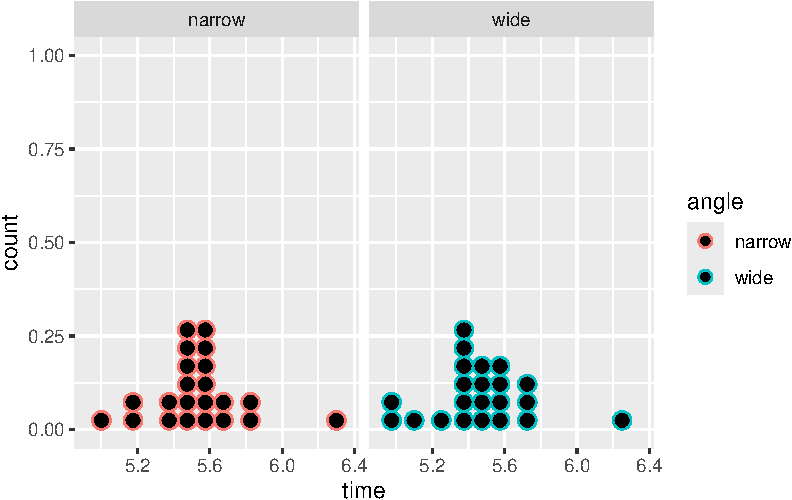
\includegraphics{Section4-One-Pred-Two-Levels_files/figure-pdf/bases-plot-1.pdf}

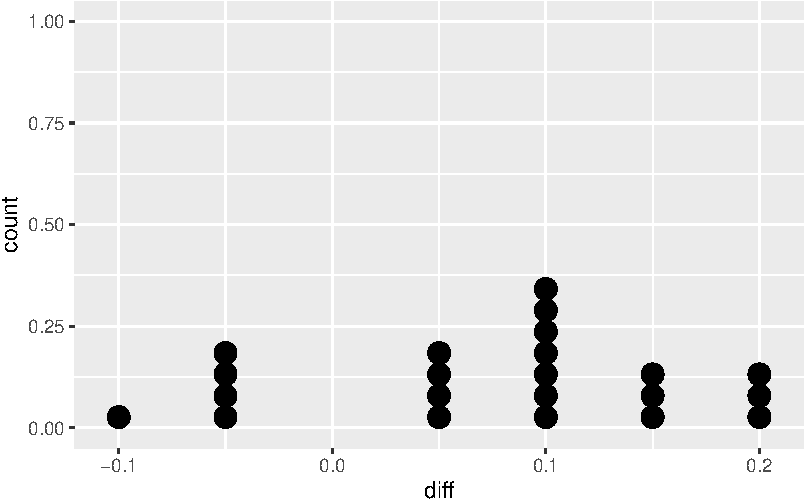
\includegraphics{Section4-One-Pred-Two-Levels_files/figure-pdf/diff-plot-1.pdf}

\begin{verbatim}
[1] 0.075
\end{verbatim}

Parameter of interest:

Hypotheses of interest:

\hfill\break
\hfill\break
\hfill\break
\hfill\break

Observed statistic:

Like before, we're trying to determine if it's surprising to see such a
large difference as \(\bar x_d = 0.075\) just by chance, if running
strategy has no effect on running time.

\begin{Shaded}
\begin{Highlighting}[]
\FunctionTok{t.test}\NormalTok{(bases}\SpecialCharTok{$}\NormalTok{diff)}
\end{Highlighting}
\end{Shaded}

\begin{verbatim}

    One Sample t-test

data:  bases$diff
t = 3.9837, df = 21, p-value = 0.0006754
alternative hypothesis: true mean is not equal to 0
95 percent confidence interval:
 0.03584814 0.11415186
sample estimates:
mean of x 
    0.075 
\end{verbatim}

\begin{Shaded}
\begin{Highlighting}[]
\FunctionTok{t.test}\NormalTok{(time}\SpecialCharTok{\textasciitilde{}}\NormalTok{angle,}\AttributeTok{data=}\NormalTok{bases2)}
\end{Highlighting}
\end{Shaded}

\begin{verbatim}

    Welch Two Sample t-test

data:  time by angle
t = 0.93383, df = 41.899, p-value = 0.3557
alternative hypothesis: true difference in means between group narrow and group wide is not equal to 0
95 percent confidence interval:
 -0.08709334  0.23709334
sample estimates:
mean in group narrow   mean in group wide 
            5.534091             5.459091 
\end{verbatim}

\subsection{Comparing Variances}\label{comparing-variances}

Often it is useful to test if variances from independent populations are
different. For example,

\begin{itemize}
\item
  a geneticist wants to test equality of the genotypic variances of
  kernel weight of two different corn populations
\item
  an engineer is interested in comparing the process variance of two
  different types of production systems used to make a electronic
  component
\item
  the two-sample \(t\)-test is based on the assumption that the
  variances of the two populations are equal
\end{itemize}

Assume the data from both populations follow a normal distribution with
different means and possibly different variances. We want to test

\hfill\break
\hfill\break
\hfill\break
\hfill\break

A natural approach would be to take samples of \(n_1\) and \(n_2\)
observations from the two populations, and compute \(s_1^2\) and
\(s_2^2\). We could then take the ratio \(s_1^2/s_2^2\) and reject
H\(_0\) if the ratio is very different from 1. But, we need to know the
sampling distribution of the ratio \(S^2_1/S^2_2\). Recall

\hfill\break
\hfill\break
\hfill\break
\hfill\break

\newpage

Sir R. A. Fisher showed that the ratio of two independent \(\chi^2\)
distributions has an \(F\) distribution with \((n_1-1)\) and \((n_2-1)\)
degrees of freedom. Specifically,

\hfill\break
\hfill\break
\hfill\break
\hfill\break

Under H\(_0: \sigma^2_1 = \sigma^2_2\) then

\hfill\break
\hfill\break

The \(F\) distribution

\begin{itemize}
\tightlist
\item
  is non-negative, unimodal, and right skewed
\end{itemize}

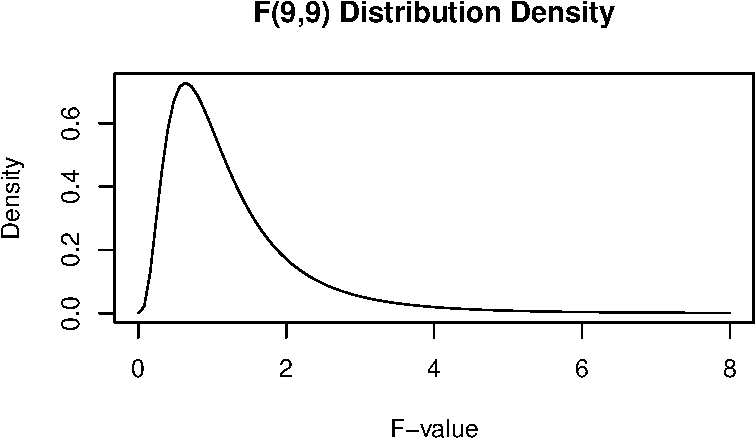
\includegraphics{Section4-One-Pred-Two-Levels_files/figure-pdf/F-distribution-1.pdf}

\begin{itemize}
\tightlist
\item
  the shape of the distribution depends on the numerator and denominator
  degrees of freedom
\end{itemize}

So, to test H\(_0: \sigma_1^2 = \sigma_2^2\) versus
H\(_a: \sigma_1^2 \neq \sigma_2^2\), we can

\begin{itemize}
\item
  Assume that \(S_1^2\) is the larger of the two sample variaces
\item
  Use \(S_1^2/S_2^2\) as a test statistic. Under H\(_0\), this ratio
  will follow an \(F\) distribution with \(n_1-1\) and \(n_2-1\) degrees
  of freedom
\item
  Use the \(F\) distribution to see if \(s_1^2/s_2^2\) is enough bigger
  than 1 to convince us the null hypothesis is not true (always a
  right-tail test!)
\end{itemize}

\textbf{Example:} The writings of different authors can be partially
characterized by the variablity in the lengths of their sentences. Two
manuscripts, \(A\) and \(B\), are found by a historian and they want to
know whether they have the same author. Fifteen sentences from each are
chosen at random, and word counts per sentence are recorded. The
historian finds \(s_A^2= 0.114\) and \(s_B^2= 0.143\).

\hfill\break
\hfill\break
\hfill\break
\hfill\break
\hfill\break
\hfill\break
\hfill\break
\hfill\break
\hfill\break
\hfill\break
\hfill\break
\hfill\break
\hfill\break
\hfill\break
\hfill\break
\hfill\break

We can use \texttt{var.test()} in R, but must have the whole data set.

\textbf{Example:} Earlier, we used a data set with nutrition levels in
people's blood as well as information about their eating habits that
came from a random sample of 315 US adults.

\begin{Shaded}
\begin{Highlighting}[]
\NormalTok{NutritionStudy}\OtherTok{\textless{}{-}}\FunctionTok{read.csv}\NormalTok{(}\StringTok{"NutritionStudy.csv"}\NormalTok{,}\AttributeTok{header=}\ConstantTok{TRUE}\NormalTok{)}

\FunctionTok{head}\NormalTok{(NutritionStudy)}
\end{Highlighting}
\end{Shaded}

\begin{verbatim}
  ID Age Smoke Quetelet Vitamin Calories  Fat Fiber Alcohol Cholesterol
1  1  64    No  21.4838       1   1298.8 57.0   6.3     0.0       170.3
2  2  76    No  23.8763       1   1032.5 50.1  15.8     0.0        75.8
3  3  38    No  20.0108       2   2372.3 83.6  19.1    14.1       257.9
4  4  40    No  25.1406       3   2449.5 97.5  26.5     0.5       332.6
5  5  72    No  20.9850       1   1952.1 82.6  16.2     0.0       170.8
6  6  40    No  27.5214       3   1366.9 56.0   9.6     1.3       154.6
  BetaDiet RetinolDiet BetaPlasma RetinolPlasma    Sex VitaminUse PriorSmoke
1     1945         890        200           915 Female    Regular          2
2     2653         451        124           727 Female    Regular          1
3     6321         660        328           721 Female Occasional          2
4     1061         864        153           615 Female         No          2
5     2863        1209         92           799 Female    Regular          1
6     1729        1439        148           654 Female         No          2
\end{verbatim}

The Quetelet index is a measure of body mass (BMI). Suppose we are
interested in whether smokers and nonsmokers have the same variability
of BMI scores.

\hfill\break
\hfill\break
\hfill\break
\hfill\break

\begin{Shaded}
\begin{Highlighting}[]
\FunctionTok{var.test}\NormalTok{(Quetelet}\SpecialCharTok{\textasciitilde{}}\NormalTok{Smoke,}\AttributeTok{data=}\NormalTok{NutritionStudy)}
\end{Highlighting}
\end{Shaded}

\begin{verbatim}

    F test to compare two variances

data:  Quetelet by Smoke
F = 1.563, num df = 271, denom df = 42, p-value = 0.08157
alternative hypothesis: true ratio of variances is not equal to 1
95 percent confidence interval:
 0.9438906 2.3908039
sample estimates:
ratio of variances 
          1.563047 
\end{verbatim}

Now that we've covered one predictor variable with two levels, we can
move on to one predictor variable with more than 2 levels.




\end{document}
